	The term "generaliZability" is used widely in literature, despite rarely being particularly well defined. Often, generalizability refers merely to the state of a predictor as "not overfitted". In other words, that it maintains sufficient performance across the training, validation, and test-sets. This, however, typically neglects the more salient aspects of the performance of the pipeline; namely how it behaves when deployed in practical settings, on data that may be distributed differently from the training dataset. Consider for instance the problem of detecting and classifying traffic signs. Though it is relatively trivial to achieve decent performance on such a task when training and evaluating on one specific dataset, it is another matter entirely to make sure the resulting predictors are robust to any and all forms of variability one might expect to see when deployed in a practical setting. If the training data was for instance collected from a region with a dry, temperate climate, it might not come as a surprise that it will not perform as well when deployed in an area prone to snowfall, fog, or generally low visibility. Of course, this could be mitigated by ensuring that the training data contains samples from a wide variety of climates, but this really only affects the robustness of the pipeline to differing climates. It does not necessarily ensure that the resulting predictors learn to ignore weather effects entirely, and as such it may nonetheless fail if it encounters something it has not been explicitly trained on. This is made especially evident in the study of black-box adversarial attacks: %examples ...
	        
	In other words, merely being robust to a limited class of perturbations or variability is not sufficient to deem a pipeline as generalizable. The pipeline must not merely learn to be right, but right for the right reasons. If this is achieved, robustness to distributional shifts follows. The system outlined above should in other words not only be robust to snow or rain or fog, but to be able to ignore the effects thereof entirely. A perfectly generalizable pipeline shouuld return a weather-invariant predictor every time, and for that matter maintain invariance to any and all non-destructive distributional shifts. 
	        
	The term generalizability will as such in this thesis refer to the ability to infer the right inductive biases from an incomplete dataset. This is as opposed to robustness, which denotes the ability of a pipeline to maintain its performance across certain distributional shifts. Generalizability is as a consequence not as much of a measurable quantity as much as it is an emergent property of a well-designed pipeline. 
	        
	This section will explore the concept of generalizability in further detail. It will outline how typical deep learning-based systems aim to achieve generalizability, why it nonetheless often fails to do so, and how one can analyse such generalizability failure.
	
			Naturally, however, real-world data is rarely neat enough for it to consistently abide by the iid assumption. Commonly encountered variation in real world data such as variable lighting conditions, class imbalance, image corruptions, noise, or other more subtle forms of distributional shift all result in structural misalignment of the training and deployment distributions (citation). Ideally, predictors should be robust to these sorts of changes, however evidently this is in not guaranteed by ERM (citation). ERM simply guarantees an iid-optimal predictor. While the difference is subtle, it is worth reemphasizing: empirical risk minimization only generalizes to data which is more or less identically distributed to the training data. Differently distributed or otherwise perturbed data, even that which is near imperceptible or at any rate inconsequentially different to the human eye, violates the iid assumption, and can as such not be expected to be classified correctly given a predictor trained via ERM. 
	
	To mitigate this, one could simply add more data to the pipeline through augmentation, or simply collecting more training data. This will lead to a better approximation of the true risk. This does not, however, solve the problem. The variability of the real world is not, unfortunately, easy to model merely through augmentations, and collecting sufficient data to cover every potential source of natural variability is infeasible, especially in medical domains. 
	%link this
	Consider for example a machine-learning pipeline wherein a model is trained to classify cows and camels. The dataset consists of cows, pictured in grass fields and pastures, and camels, pictured in deserts. To be generous, let us assume that we have sufficient quantities of data to ensure that the pipeline is perfectly invariant to the pose of the respective animals, to lighting conditions, geometric transforms, etc. One may then expect that the pipeline correctly learns to classify the two, and attains high accuracies, and indeed when evaluated on iid data, this would be entirely correct. However, what would then happen if one such predictor encountered a cow in the desert and a camel in a grass pasture? This constitutes a distributional shift, and as such we cannot expect reliable performance as detailed in \ref{erm}. Naturally, the predictor may have learned just fine exactly what constitutes a cow and a camel, but it might just as easily learned to associate deserts with camels and pastures with cows. And from a data perspective, both are equally correct interpretations. The immediate response to this may be to simply add some pictures with more varied backgrounds, but this once again would only serve to make the pipeline more robust to backgrounds. it would not guarantee that the pipeline learns the right inductive biases. The predictor may then for example instead learn that cows typically are black and white and camels usually beige, and then fail when it encounters a brown cow. One could keep adding more and more data, but there is not really any way of knowing when the pipeline is well enough specified by the data such that it starts returning predictors with the desired inductive biases. There are in simpler terms several "correct" interpretations of what separates the classes from a purely data-based perspective, each with their own inductive biases. There are as a consequence not just one risk-minimizing predictor, but a whole family of them. This is referred to as underspecification \cite{damour2020underspecification}.
	
	
		\subsubsection{Overfitting and underfitting}
	Overfitting and underfitting are perhaps the two most well-understood instances of generalisation failure. In simple terms, underfitting occurs when the span of the hypothesis space is insufficient to adequately model the relationships the model is intended to capture. Simple linear regression would, for instance, always fail to produce a generalisable predictotor of non-linear relationships between its input variables. Similarily, a neural network may be too shallow or too short, in which case the pipeline can never, even given infinite data and an optimal optimization process, find \(f\), since it simply does not exist in \(\mathcal{H}\) This is of course a fairly trivial problem to solve: simply increase the depth and/or width  of the model. And indeed, this is principally the reason why deep learning networks have proven to be superior to its more simple counterparts.
	

	Generalization failure is then in this case and by this line of reasoning entirely dependent on the structural misalignment and distributional shift corresponding to the change in imaging techniques as opposed to any erroneous logic in the pipeline itself. Ideally, the pipeline should of course detect patterns that generalize well regardless of lighting conditions, but it is not reasonable to expect the pipeline to draw this conclusion autonomously. Instead, the pipeline has to be "told" to keep this invariance in mind during training a priori. If some hypothetical change to the pipeline were to manage to induce this invariance, the structural misalignment between the dataset would no longer be an issue, ceteris paribus.

	The behavior that violations of assumptions \ref{underfit} and \ref{overfit} is well understood and fairly easy to detect, corresponding to underfitting and overfitting respectively, but violations of the remaining assumptions result in more subtle forms of generalization failure. 
		
	The general consensus is that generalization
	failure can in broad strokes be attributed to either underspecification or structural misalignment. The following sections will attempt to summarize and synthesize the analyses within the literature, and connect each of the generalization
	failure modes they identify to the above violations.

	In broad strokes, the generalisation failure modes identified in the literature can be categorized as belonging to one of the following phenomena:
		\begin{itemize}
			\item Pareidolia
			\item Underspecification
			\item Causal agnosticism 
		\end{itemize}
		
		, consider the problem of classifying images of cows and camels as the respective animals, wherein the dataset consists of images of cows in grass fields and pastures, and camels in deserts. To be generous, let us assume that we have sufficient quantities of data to ensure that the pipeline is perfectly invariant to the pose of the respective animals, to lighting conditions, geometric transforms, weather, etc. One may then expect that the pipeline correctly learns to classify the two, and attains high accuracies, and indeed when evaluated on iid data - i.e cows in fields and camels in deserts, this would be correct. However, what would then happen if one such predictor encountered a cow in the desert and a camel in a grass pasture? This, of course, constitutes a distributional shift, and as such we cannot expect the models to generalize. The predictor may have learned just fine exactly what constitutes a cow and a camel, but it might just as easily have learned to associate deserts with camels and pastures with cows. And from a purely statistical perspective, both are equally correct interpretations. From a causal perspective, however, it is of course entirely nonsensical to assume the respective animals are wholly defined by their surroundings.


		As described in earlier sections, good generalizability can only be achieved if the pipeline can reliably generate predictors that learn causally reasonable features and consequently encode robust inductive biases. Naturally, knowing what features are causal and which are confounding is an intractable problem; otherwise generalization would simply be a matter of precisely expressing the right inductive biases algorithmically, through conventional image analysis. As a result, it is instead necessary to consider what constitutes are \texit{non-robust} features, and ensure that the model does not try to leverage these features during prediction. 

		To achieve this, a model of natural variation (MNV) is constructed, which aims to encapsulate the variability one might expect to see in the domain. This model can then be leveraged to force the DNN to be robust to the space of transformations that it defines. It is of course impossible to fully encapsulate all the possible variability one may see in the wild, but that is not necessarily obligatory so long as the search space is limited to areas wherein robust features are required. The key idea here is that it is more likely that the model learns causally viable features, than spurious features that somehow nonetheless exhibit invariance to a large space of transformations. 
		
		The construction of such a model is of course not necessarily trivial. The MNV has to be non-destructive - i.e, the model should not transform the input beyond recogniton - yet it cannot be too lenient either. The model should optimally also not affect the properties of the image that correspond to causal structure. To give a simple example: a model that classifies hand-written digits should not be invariant to rotation, as the orientation of the number 6 or 9 has causal significance, and should consequently not be included in a MNV. For more complex tasks, designing this model therefore requires some supervision - if the image at any point becomes difficult to distinguish to the human eye, the augmentations are too severe. 
	
		There are also several possible approaches as to how such a model can be leveraged. In this thesis, these approaches are as follows:
		\begin{itemize}
			\item MNV as data augmentation
			\item MNV consistency training
			\item Adversarial MNV consistency training
		\end{itemize}
	
		The reasoning behind this is that consistent behaviour should be rewarded even if the model has not quite learned how to perform to an adequate standard, as this is preferable to merely learning to perform well without any regard for consistency and by extension causality.  To illustrate, consider once more the example from chapter \ref{background}, namely the problem of acheiving generalisation from narrow-band to white-light imaging datasets and vice versa. Assume that the perturbation function simply maps between the respective lighting modalities. In this case, the loss will reward the model if it predicts identical segmentations regardless of lighting conditions, even if the predictions are incorrect. The model will nevertheless be trying to leverage features which are invariant to lighting, and consequently be more generalizable than a pipeline wherein the model is permitted to be leverage lighting-dependent features.


		Overfitting occurs when the model learns patterns that are too complex to be likely to actually describe the process(es) that generate them. Once again, to give a somewhat simple example: 
		\begin{figure}[h]
			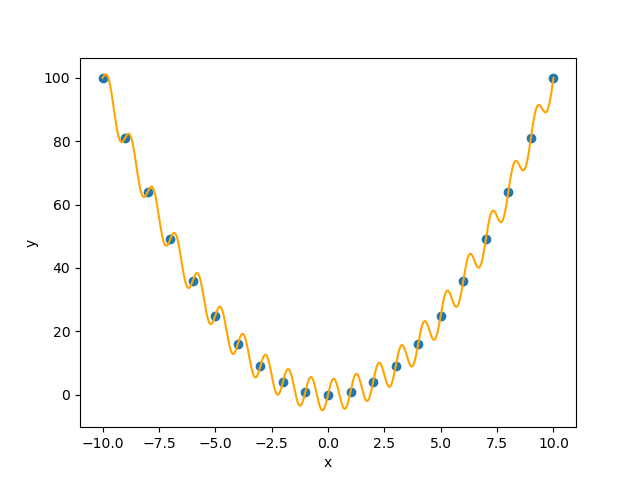
\includegraphics[width=\linewidth]{illustrations/overfit.png}
			\caption{A model with excessive capacity interpolates unneccesarily complex patterns}
			\label{Overfit example}
		\end{figure}
		The underlying function is once again \(y=x^2\). The sinusoidal pattern in the interpolated function is obviously erroneous, but this is impossible to determine with complete certainty given only a finite sampling of the underlying function. More generally, every finite sampling of any function can be interpolated as any one of an uncountably infinite set of functions. To prove this, consider the task of finding a function that fits the series \((1,4,9)\). Though ones first instinct would be to assume the pattern is described by the function \(y=x^2\), and that the next number in the sequence thus is 16, the next number can really be anything at all. Using Newton interpolation, or for that matter any arbitrary interpolation scheme, one can easily find a polynomial that fits the sequence \((1,4,9,n, n \in \mathbb{R}\). Since the set of real numbers is uncountably infinite, it follows that the space of functions that fits this new sequence also is uncountably infinite, depending on \(n\). Thus, there is an uncountably infinite number of functions that describe \(1,4,9\) as well. This of course does not only apply to extrapolating the next element in a sequence, but also any interpolating between consecutive elements. 
		Naturally, this logic also applies to neural networks. Though instead of discrete sequences, it is probability distributions that are being modelled. Just like how extrapolation and interpolation between points is ill-defined for sequences, it is ill-defined for probability distributions.
		
		Consequently, it is necessary to introduce a number of assumptions and constraints to the problem. (CLARIFY)
		
		Obviously, the minimum level of generalization one should achieve is generalization to iid data. To this end, it is necessary to incorporate an iid evaluation method, such as keeping hold-out sets, cross validation, etc. This is of course ubiquitous in modern deep learning. Moreover, it is necessary to make some assumptions regarding the simplicity - or rather, complexity - of the resulting predictor. Certain neurons should for instance not dominate the predictions, the weights should have reasonable values, etc. This is what motivates so-called regularization, whereby different methods - for instance batch normalization, drop-out, L2 loss, weight decay, etc - are used to bias the search towards areas in the loss landscape that are more credible from a perspective of model complexity. This is of course only necessary because assumptions \ref{overfit} and \ref{underspecification} do not hold. Given a perfect (or at least very well sampled) representation of the risk and consequently the loss-landscape and a perfect optimizer, the model would not overfit in any meaningful way.  

		Regularization has of course for this reason been extensively studied, and for most purposes the existing regularization techniques suffice just fine for IID data, and typically yield highly performant predictors so long as it is not subjected to any form of distributional shift. Consequently, Overfitting, though naturally still a factor that needs to be accounted for when designing deep learning pipelines, is not at fault for the generalization failure that is exhibited in modern deep learning systems.

\section{Consistency Loss}
Similarly to how one can optimize for the Jaccard Index through the Jaccard Loss, so too can one optimize for consistency by using SIC as a component of a loss function. Naturally, using SIC on its own is not really useful since it only expresses consistency, and is wholly agnostic to whatever object it is trying to segment. Consequently, it has to be combined with a some conventional segmentation loss. A simple way to do this would be to simply add them together and normalize, i.e:
\begin{equation*}
    L(Y, A) = \frac{1}{2} \big[L_{seg}(Y)+L_c(Y,A)\big]
\end{equation*}
Preliminary experiments showed that this, however, exhibited some degree of instability. The model would readily get stuck in local minima where its predictions were indeed consistent, but also consistently predicting artifacts. Examples of this can be found in the appendix. To mitigate this, a better loss function is required. Instead of simply adding the respective losses together, one may weight the individual components adaptively according to the segmentation performance. This way, the model will learn generally correct interpretations early in the training, then start weighing consistency more and more as the model sees improvements to its segmentation performance:
    \begin{equation}
        L = (1-IoU)\times L_{seg} + IoU \times L_c
    \end{equation}
        If the Jaccard Index (IoU) is used, this is also equivalent to:
    \begin{equation}
        L = {L_{jac}}^2 + (1-L_{jac})\times L_c
    \end{equation}
Using this formulation, the model will start off trying to learn features that contribute to generally improved segmentation performance, then as segmentation performance improves start principally focusing on learning consistent features. Moreover, if the model starts veering into areas in the loss-landscape that constitute poor segmentation performance, it will self-correct by weighing the segmentation loss more. 

\begin{center}
        \begin{tabular}{|c|c|c|c|c|}
        \hline
        \multicolumn{5}{|c|}{\textbf{DeepLab}}\\
        \hline
        &\multicolumn{4}{|c|}{Datasets}\\
        \cline{2-5}
        Configuration&HyperKvasir&Etis-LaribDB&EndoCV2020 & Clinic-CVC \\
        \hline
        Vanilla& 0.828 & 0.453 & &\\
        \hline
        \(\epsilon\)-Augment& 0.833 & 0.508 & 0.682 & 0.711 \\
        Consistency & 0.847 & 0.553 & 0.697 & 0.727 \\
        Adversarial Consistency & 0.844&0.524&0.696&0.726 \\
        Weighted Jaccard&0.850&0.531&0.699&0.731\\
        \hline
        \multicolumn{5}{|c|}{\textbf{FPN}}\\
        \hline
        &\multicolumn{4}{|c|}{Datasets}\\
        \cline{2-5}
        Configuration&HyperKvasir&Etis-LaribDB&EndoCV2020 & Clinic-CVC \\
        \hline
        Vanilla&  &  & &\\
        \hline
        \(\epsilon\)-Augment& & & & \\
        Consistency & & && \\
        Adversarial Consistency&&&& \\
        Weighted Jaccard&&&&\\
        \hline
        \multicolumn{5}{|c|}{\textbf{UNet}}\\
        \hline
        &\multicolumn{4}{|c|}{Datasets}\\
        \cline{2-5}
        Configuration&HyperKvasir&Etis-LaribDB&EndoCV2020 & Clinic-CVC \\
        \hline
        Vanilla&  &  & &\\
        \(\epsilon\)-Augment& & & & \\
        Consistency & & && \\
        Adversarial Consistency&&&& \\
        Weighted Jaccard&&&&\\
        \hline
        \multicolumn{5}{|c|}{\textbf{Tri-Unet}}\\
        \hline
        &\multicolumn{4}{|c|}{Datasets}\\
        \cline{2-5}
        Configuration&HyperKvasir&Etis-LaribDB&EndoCV2020 & Clinic-CVC \\
        \hline
        Vanilla&  &  & &\\
        \(\epsilon\)-Augment& & & & \\
        Consistency & & && \\
        Adversarial Consistency&&&& \\
        Weighted Jaccard&&&&\\
        \hline
        \end{tabular}
    \end{center}
    
            \begin{figure}[h]
            \centering
            \begin{tabularx}{\linewidth}{XXXXXXXXXX}
            \toprule
            \multicolumn{10}{c}{\textbf{No Augmentations, Vanilla Training, Jaccard evaluation}}\\
            \toprule
            &&\multicolumn{2}{c}{HyperKvasir} &
            \multicolumn{2}{c}{Etis-LaribDB} & 
            \multicolumn{2}{c}{Clinic-CVC} & 
            \multicolumn{2}{c}{EndoCV2020}\\
            \cmidrule(lr){3-4}\cmidrule(lr){5-6}            \cmidrule(lr){7-8}\cmidrule(lr){9-10}
            && IoU & \(SIS_{auc}\) & IoU & \(SIS_{auc}\) &IoU & \(SIS_{auc}\) & IoU & \(SIS_{auc}\) \\  
            \midrule
            \multicolumn{2}{c}{DeepLabV3+} & 0 & 0 & 0 & 0 & 0 & 0 & 0 & 0 \\
            \multicolumn{2}{c}{FPN} & 0 & 0 & 0 & 0 & 0 & 0 & 0 & 0 \\
            \multicolumn{2}{c}{UNet} & 0 & 0 & 0 & 0 & 0 & 0 & 0 & 0 \\
            \multicolumn{2}{c}{Tri-UNet} & 0 & 0 & 0 & 0 & 0 & 0 & 0 & 0 \\
            \multicolumn{2}{c}{InductiveNet} & 0 & 0 & 0 & 0 & 0 & 0 & 0 & 0 \\
            \bottomrule
        \end{tabularx}
            \caption{Model Generalizability given vanilla training, but without data augmentation, using standard loss-based \gls{ind} evaluation procedures}
            \label{table:vanilla}
        \end{figure}
        
        
    \subsection{Consistency Evaluation}
    As mentioned earlier in this thesis, the evaluation methods typically used in deep learning pipelines consider only the \gls{ind} case and presupposes that the \gls{iid} assumption holds. To investigate whether \gls{sis}-based evaluation can increase the likelihood of selecting generalizable predictor during early-stopping, the previous experiment was repeated, but instead of selecting predictors according to the minimal validation loss, they were selected according the minimal \gls{sis}-score. Once again, 10 predictors were trained for each model. The metric values for this experiment are shown in Table \ref{table:sis_eval}. For easier comparison, table \ref{table:sis_eval_delta} shows the percentage-wise change in the respective metrics. 
    
    \subsection{Siamese Consistency Training}
        The modified pipeline with Siamese Consistency Training was evaluated in a similar manner to the above experiments. Evaluation was however based on the inconsistency loss, though for the sake of completeness tables considering \gls{sis}-only evaluation are included in the Appendix. 
        
        Since this pipeline leverages augmentations, results from the vanilla pipeline, but with the incoming batch being augmented using the perturbation model, are also included in order to discern between the impact of the training routine itself and the effects of data augmentation.
        
    % Prior to Deep Learning, these sorts of problems were typically solved using complex feature- extraction and -engineering techniques, which were then given to some relatively simple classifier or regression model. These types of approaches were often lacking performance-wise, and typically fairly difficult to engineer, requiring a deep understanding of image-analysis techniques, feature engineering, and so on. Moreover, they were also fairly brittle, with a significant body of work being dedicated solely to improving preprocessing techniques such 
    
          % For computer vision problems - therein polyp segmentation - the inputs are typically images or videos, and are typically processed using a type of \gls{dnn} known as a \glsfirst{cnn}. These are based on a mathematical operation known as convolution. These convolutions process the image according to the parameters of a number of convolution kernels. The model learns these parameters by iterating over a dataset consisting of input-output pairs - for instance images and class-labels - and adjust the parameter values according by in a process known as gradient descent. This is referred to as training. The resulting trained model, often called a predictor, will then (ideally) be capable of performing inference with sufficient performance. 
        
        
        % What is deep learning
        % How does it work
        % Why is it used for polyp segmentation
        % Introduce the idea of the deep learning pipeline
        % Deep learning is a form of machine-learning, wherein the model has the capacity to model practically any data for practical purposes, so long as it is given sufficient data upon which it can "learn". Similar to how a linear-regression model can leverage some dataset to learn a linear relationship between some number of variables, a \gls{dnn} may leverage a dataset learn some arbitrary, highly non-linear relationship.
    
        % Most real-world phenomena are, naturally, fairly non-linear in nature, and as a consequence often require exceedingly complex models to be able to reason about them sufficiently. This, in part, explains the 
    
        % For the purposes of this thesis, it may be useful to think about \glspl{dnn} as general-purpose correlation machines; i.e that they take some data in, and then spits out some correlations it has managed to identify within this data. This notion will be explained in more detail later in this chapter. 
        
        % For computer vision, the most common \gls{dnn} architecture is the \gls{cnn}. \glspl{cnn} operate using convolutions, as its name suggests. These convolutions process the image according to the parameters of the convolution kernels, which the model learns during training.
        
        
        To investigate the impact of each of the components of the new pipeline, and the possible dynamics between them, an ablation study was conducted. Every combination of validation procedure, loss function and augmentation strategy were tested across a number of models. For each of these combinations, ten predictors were trained in order to test their impact to statistical significance. \autoref{experiments} shows a diagram detailing the experiments performed. For each model, a predictor was trained varying its evaluation procedure - namely \gls{sis}-based and loss-function based, for each loss function - either jaccard or \gls{sil}, and for each augmentation stategy - either no augmentation, vanilla data augmentations, and vanilla augmentations with the GAN-inpainter. Since \gls{sil} requires augmentations to work, it obviously cannot be tested without using data augmentation, and as such this configuration is dropped from the tree.

\begin{figure}[h]
    \centering
    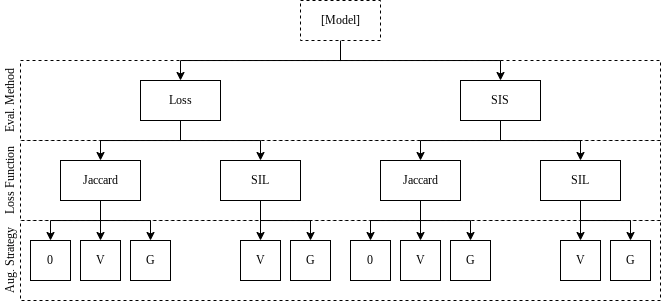
\includegraphics[width=\linewidth]{illustrations/experiment.png}
    \caption{Diagram over Experiments. 10 predictors are trained for each leaf-node in the tree. In the augmentation strategy layer, 0 corresponds to no augmentation, V to vanilla augmentation, and G to augmentation using both vanilla augmentations and an inpainter}
    \label{fig:experiments}
\end{figure} 

Since inpainting is intended to serve as an auxiliary augmentation technique on top of conventional augmentations, and due to insufficient computatational resources, it was only tested in conjunction with conventional augmentation.  

This chapter will cover in further detail how the experiments were conducted and how the methods were implemented, as well as present the results of the ablation study. Discussion and analysis of these results and their implications will be reserved for chapters \ref{analysis} and \ref{discussion}. 

          In conventional deep learning pipelines, the value of the loss function used to compute, and as a consequence the gradient, is computed from some sample of the training data. This is known as \glsfirst{erm}. The size of this sample gives rise to three different families of optimization techniques: stochastic gradient descent, which uses one training sample at a time to approximate the gradient, mini-batch gradient descent, which uses a few of the available training samples, and batch gradient descent, which uses the entire training set. This is determined by the Dataloader. Mini-batches are used in most modern deep learning pipelines, and as such this will be assumed for the rest of this section.
          Instead, the training procedure loops through the entire training set some number of times, computes the loss and the gradient, minibatch or batch, and finally update the weights according to the optimizer and scheduler by backpropagating the gradient of the loss function with respect to the relevant weights.
          
          
% OLD SUMMARY
\cref{background} provided an overview of deep learning, segmentation, and delved further into why such systems so readily fail to generalize, starting from first principles and analyzing the shortcomings of \gls{erm}. This was then connected to recent analyses of generalizability failure, including the notion of underspecification and shortcut learning. Finally, known methods of increasing generalization as presented in EndoCV2021 and elsewhere in the literature were then discussed and analysed with respect to the established theory. 

This was then in turn used to inform the development of the methods discussed in \cref{methods}, including a novel training paradigm, augmentation technique, model architecture and ensemble models. Each of these methods were also discussed with respect to the theory explored in \cref{background}.
Several experiments were then conducted in \cref{experiments} in order to ascertain the impact of the proposed methods:

First, baseline generalizability metric were collected for five separate models. The findings supported the notion that larger models are more prone to generalizability failure, as demonstrated by the significant gap between the Unet and the TriUnet. The dual-decoder DeepLabV3+ exhibited considerably lower generalizability than the regular DeepLabV3+. This suggests that underspecification may not be the principle cause of generalizability failure across these two models. As will be discussed in the next section, this merits further study.

In the next experiment, data augmentation was shown to increase generalizability by a considerable margin. Synthetic augmentation via inpainting was shown to reduce generalizability, but this finding was deemed inconclusive due to the relatively low performance of the inpainter. 

The impact of consistency training was then tested and compared to regular data augmentation and no augmentation. The results show that consistency training outperforms regular data augmentation by a considerable margin on the most difficult of the three \gls{ood} datasets. The impact on the remaining datasets was somewhat lower, however, with the difference being statistically significant only on one of them. 

Finally, predictors trained according to the best methods as identified in the previous experiments were then combined into ensembles. The results demonstrated the generalizability of ensemble-based methods and corroborated the theoretical analyses discussed in \cref{background} that this can in large part attributed to the fact that ensembles mitigate underspecification. 

The results from this experiment was then discussed in \cref{discussion}. Limitations of the experiments were noted, along with their practical impacts and possible directions of further study and means of improvement of the methods proposed in this thesis. 

\begin{align}
L_s &= \frac{1}{\sum \hat{y} \cup \hat{a}} \sum \hat{y}\ominus y \\
L_c &= \frac{1}{\sum \hat{y} \cup \hat{a}}\sum  [\hat{y}\ominus y\ominus \hat{a} \ominus a  ]\\
L_{c+s} &= L_c(Y, A) + L_s(Y)\\
&=\frac{1}{\sum \hat{y} \cup \hat{a}} \Bigg[\sum  \{\hat{y}\ominus y\ominus \hat{a} \ominus a  \} + \sum \{\hat{y}\ominus y\}  \Bigg]\\
\begin{split}
&=\frac{1}{\sum \hat{y} \cup \hat{a}} \Bigg[\sum \{\hat{y}\ominus y\} + \sum  \{\hat{a}\ominus a\}\\
&-\sum \{\setminus y\cap \hat{y} \cap a \cap \hat{a}\}\cup\{y\cap \setminus \hat{y} \cap a \cap \hat{a}\}\cup \\ 
&\{y\cap \hat{y} \cap \setminus a \cap \hat{a}\}\cup\{y\cap \hat{y} \cap a \cap \setminus \hat{a}\}\\
&-\sum\{\setminus y\cap \hat{y} \cap \setminus a \cap \hat{a}\} \cup\{y\cap \setminus \hat{y} \cap \setminus a \cap \hat{a}\} -\\
&\cup\{\setminus y\cap \hat{y} \cap a \cap \setminus\hat{a}\}\cup\{y\cap \setminus \hat{y} \cap a \cap \setminus \hat{a}\} \\ 
&+\sum \{\hat{y}\ominus y\}   \Bigg]\\
\end{split}\\
\begin{split}
&=2L_s(y, \hat{y})+L_s(a, \hat{a}) +\frac{1}{\sum \hat{y} \cup \hat{a}} \Bigg[\\
&-\sum \{\setminus y\cap \hat{y} \cap a \cap \hat{a}\}\cup\{y\cap \setminus \hat{y} \cap a \cap \hat{a}\}\cup \\ 
&\{y\cap \hat{y} \cap \setminus a \cap \hat{a}\}\cup\{y\cap \hat{y} \cap a \cap \setminus \hat{a}\}\\
&-\sum\{\setminus y\cap \hat{y} \cap \setminus a \cap \hat{a}\} \cup\{y\cap \setminus \hat{y} \cap \setminus a \cap \hat{a}\} -\\
&\cup\{\setminus y\cap \hat{y} \cap a \cap \setminus\hat{a}\}\cup\{y\cap \setminus \hat{y} \cap a \cap \setminus \hat{a}\}   \Bigg]
\end{split} \label{loss_proof}
\end{align}

\begin{figure}[h]
    \centering
    \hspace*{-1.9cm}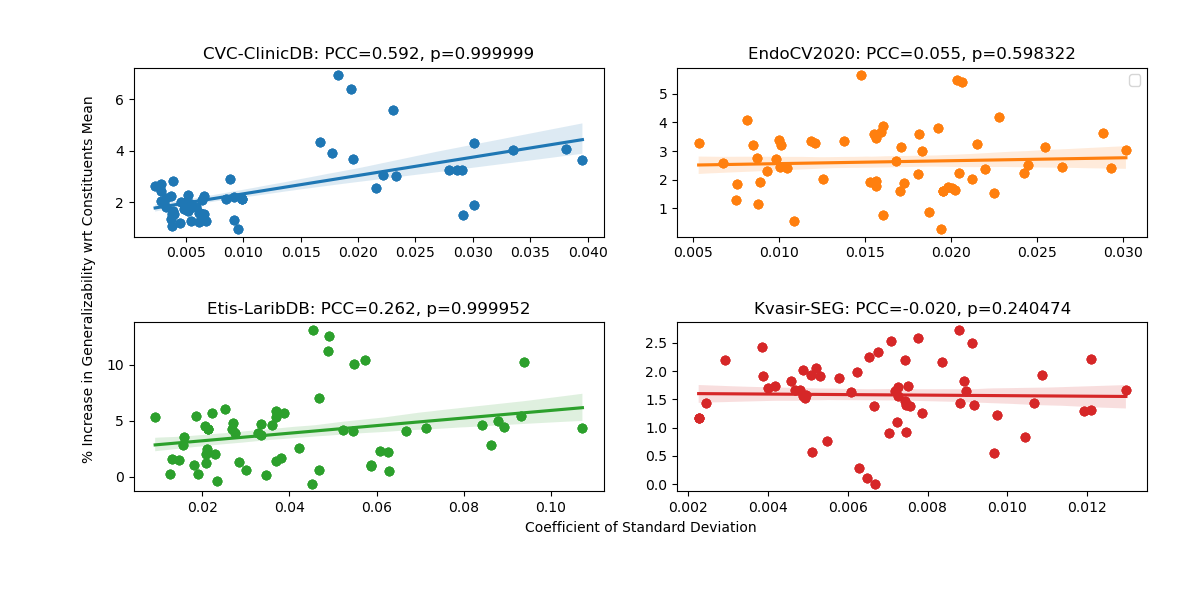
\includegraphics[width=1.2\linewidth]{illustrations/ensemble_variance_relationship_statistical.png}
    \caption[Relationship between ensemble improvements and constituents' performance variability]{Plot showing the correlation between the improvements to \gls{iou} with respect to the mean \gls{iou} of the constituent predictors, versus the variability in the performance of the constituent predictors. The Pearson Correlation Coefficient and corresponding p-value for each dataset is shown in the title of each subplot.}
    \label{fig:ensemble_var}
\end{figure}

The results do not appear to completely corroborate this analysis of why ensembles increase generalization, however. Though a Pearson correlation test reports positive correlations (p>0.99) on two of the datasets - CVC-ClinicDB and Etis-LaribDB - the relationship is nonetheless fairly spurious. This is likely to be due to the the nature of the landscape of the Bayesian posterior, as illustrated in \Cref{fig:bayesian_generalization} in \Cref{fig:bayesian_generalization}. Moreover, performance variability may not be an accurate representation of the degree to which the ensembles' constituent predictors encode different features. This will be discussed further in \Cref{discussion}. 

    \item Ensembles models increase generalization. The relationship between ensemble models and underspecification as quantified in this thesis is also somewhat more spurious than expected.
    
    However, the notion that this improvement arises as a result of mitigating underspecification was shown to not be as strong as the analyses in the literature often suggest. As shown in \Cref{fig:ensemble_var}, the relationship between improvements afforded by the use of ensembles and the degree of underspecification of the constituent model(s) is spurious. 
    
        % The improvements due to the use of ensembles was, however, comparatively minor. As discussed in previous sections, data augmentation and consistency training proved to be more effective by significant margins. On the Etis-LaribDB dataset, conventional data augmentation provided improvements to generalization ranging between 10\% and 20\%, and consistency training between 20\% and 26\% when averaging across models. Ensemble models, on the other hand,  ralization by a minor amount and at best facilitating a 13\% increase on the TriUnet.  The potential gains from ensemble models is nevertheless significant, but it should be noted that the ensembles' cost of training time, time required for inference, and the comparatively high memory requirements needs to be weighted against the benefits. It may, for instance, be the case that the computational resources spent training multiple models for use in an ensemble would be better spent tuning the augmentation strategy, which as established has a more considerable effect. 
        
\section{Future Work}
There are a myriad of promising directions for further work. These are detailed in \Cref{discussion} and can be summarized as follows:

There are several ways to improve Consistency Training. One may for instance modify the segmentation inconsistency loss as outlined in \Cref{new_closs}. It is also possible to incorporate the notion of consistency in more advanced pipelines, such as through denoising networks as outlined in \Cref{denoising}. Adversarial sampling of perturbations or otherwise modifying the perturbation model may also have merit.  

Further investigating the effect of multiple-decoder models may also prove insightful, in particular as a countermeasure to underspecification. Analyzing the latent representations and the differences that these decoders induce may also provide a better understanding of what the encoders actually learn, and corroborate the hypothesis made in \Cref{models} that they learn dataset- and thus task-invariant features. 

Repeating the experiments performed in this thesis without pretraining may also be interesting. There may for instance be a relationship between pretraining and the aforementioned tendency of encoders to learn task-independent features which such experiments would highlight.  

As this thesis merely explored the impacts of model architectures, data augmentation and ensemble models on a surface level, there is naturally space for more in-depth exploration of the relationships suggested by the findings in \Cref{experiments}. In particular, a more in-depth analysis of the impact of data augmentation is warranted, in particular in regards to the relative impacts thereof in comparison to other methods. A meta-analysis of the findings in EndoCV2021 wherein the same augmentation method is kept across all submitted methods may for instance be a useful point of further study towards developing more robust experimental methods to evaluate generalization. 


% \section{Summary}
% The goal of this work has been to develop novel methods of increasing the generalizability of deep learning models, as well as to further the understanding of the relative impacts of more conventional components of the deep learning pipeline.

% Several methods were proposed to this end, namely DD-DeepLabV3+, Consistency Training, generative polyp inpainting, and the use of ensembles. Among these methods, Consistency Training had the most significant impact and appears to be the most promising with regards to further development. 

% There are a multitude of improvements that could be made for every tested method, and there is much to be gained from more in-depth analysis and experimentation with regards to the relative impacts of all tested methods. 

% Though generalizability remains an open and multifaceted problem, there are evidently multiple promising directions of further study which may yet prove to alleviate generalization failure or at the very least facilitate a deeper understanding of generalizability. In particular, Consistency Training, and in general notion of perturbation consistency, exhibits significant potential towards mitigating generalization failure.

    
    
    % \subsubsection{Generalizability Gap}
    % Solely considering \glspl{iou} may be misleading, however ~\cite{metric_weakness}. A predictor which exhibits \glspl{iou} of 0.7 regardless of the dataset should for instance be considered more generalizable than one which scores IoUs of 0.9 or higher on \gls{iid} datasets but 0.7 on \gls{ood} datasets. Though considering the \glspl{iou} themselves is obviously for the best when considering more practical perspectives - i.e., how the system would fare in clinical deployment - a more informative measure of the ability of a given predictor to generalize is the difference between \gls{ood} and \gls{ind} performance as a percentage of its \gls{ind} performance. In the context of segmentation, this can be quantified via \gls{iou} as:

    % \begin{equation}
    %     \Delta\%IoU = 100\frac{IoU_{ind}-IoU_{ood}}{IoU_{ind}}
    % \end{equation}

    % This has the advantage of facilitating more direct comparisons of generalizability even if the models in question exhibit fairly different performance in terms of \gls{iou} also in \gls{ind} settings. 